%                                                                 aa.dem
% AA vers. 8.2, LaTeX class for Astronomy & Astrophysics
% demonstration file
%                                                       (c) EDP Sciences
%-----------------------------------------------------------------------
%
%\documentclass[referee]{aa} % for a referee version
%\documentclass[onecolumn]{aa} % for a paper on 1 column  
%\documentclass[longauth]{aa} % for the long lists of affiliations 
%\documentclass[rnote]{aa} % for the research notes
%\documentclass[letter]{aa} % for the letters 
%\documentclass[bibyear]{aa} % if the references are not structured 
% according to the author-year natbib style


\documentclass[referee]{aa}
%\documentclass{aa}

%
\usepackage{graphicx}
\usepackage{siunitx}
%%%%%%%%%%%%%%%%%%%%%%%%%%%%%%%%%%%%%%%%
\usepackage{txfonts}
%%%%%%%%%%%%%%%%%%%%%%%%%%%%%%%%%%%%%%%%
%\usepackage[options]{hyperref}
% To add links in your PDF file, use the package "hyperref"
% with options according to your LaTeX or PDFLaTeX drivers.
%
\begin{document} 
    \title{Determination of Perseid Meteoroid Flux from Meteor Data Debiased by Numerical Simulation}
    \subtitle{I. }

    \author{
        M. Baláž\inst{1}\fnmsep\thanks{martin.balaz@fmph.uniba.sk}
        \and
        J. Tóth\inst{1}
        \and
        P. Vereš\inst{2}
        \and
        R. Jedicke\inst{3}
    }

    \institute{
        Comenius University in Bratislava,
        Mlynská dolina, 84248 Bratislava, Slovak Republic \\
        \email{martin.balaz@fmph.uniba.sk} \\
        \email{juraj.toth@fmph.uniba.sk}
        \and
        Minor Planet Center \\
        \email{peter.veres@cfa.harvard.edu}
        \and
        University of Hawaii \\
        \email{jedicke@hawaii.edu}
    }

   \date{Received September 15, 1996; accepted March 16, 1997}

% \abstract{}{}{}{}{} 
% 5 {} token are mandatory

\abstract{ %
    Deployment of multi-station video meteor networks presents a unique opportunity to measure
    the total mass flux of meteoroids impinging on the surface of the Earth. However, direct measurement
    of particle flux is not possible as the data are heavily distorted by selection bias. We present
    a method for debiasing the data using a simulation of meteoroid particles entering the atmosphere
    and its reference implementation.
}{ % aims
    To develop methods of debiasing ground-based meteor observations performed with all-sky cameras
    nd to use the obtained data to determine the total particle and mass influx.
}{ % methods
    A population of meteoroid particles with known chemical composition, population index and orbital elements
    is created above the Earth's atmosphere.
    The trajectory of each virtual meteoroid is tracked and after application of selection bias
    the resulting meteor observation is recorded.
    Once a sufficiently large dataset is obtained, statistical tests
    are performed and the distributions are compared to observational data from the AMOS camera network.
    The entire procedure is repeated and the parameters of the simulation are gradually adjusted until
    best possible agreement with observational data is found.
}{ % results
    To be added later.
}{ % conclusions
    None so far.
}
\keywords{meteoroids -- meteors -- debiasing}


\titlerunning{Debiased Perseid Meteor Flux}
\maketitle
%
%________________________________________________________________

\Epigraph{
    Throughout the ages \\
    Of iron, bronze and stone \\
    We marvelled at the night sky \\
    And what may lie beyond
}{
    Children of the Sun \\
    \textsc{Dead Can Dance}
}


Research of interplanetary matter -- and meteoroids in particular -- 
... \todo{finish the sentences}



In comparison to other fields astronomy it does not produce spectacular findings too often.
The recent discoveries of exoplanets, detection of gravity waves or pictures of black holes seem to be much more fascinating.
However, deep space can only be observed, but not touched, and will continue to remain
inaccessible to us for a very long time -- if not forever.

With the Solar System, our nearest space neighbourhood, it is different. We are already able not only to observe,
but to reach it directly with our probes and -- probably within foreseeable future -- visit in person.
No matter how fast or unimaginably advances the technological progress will be, it will always be our home.
This is why now, when the technology and our knowledge are already sufficient to explore, map and possibly exploit
the nearest space, we should try hard to deepen and broaden our understanding of our cosmic home, its origin and our place in it.

\section{The need to know} \label{in}

    Like many other objects, creatures or phenomena, our nearest space is not only beautiful and interesting, but often
    also dangerous and inscrutable.

    \todo{glue}



    In a vast majority of cases, meteoroids do not pose immediate danger to human activities.
    On the surface we are shielded by the Earth's atmosphere, a layer of gases several tens of kilometres
    thick, which offer massive resistance to any object trying to enter it at high speeds.
    Only a minuscule fraction of bodies are tough and massive enough to survive the violent atmospheric entry.
    Even then, atmospheric drag slows most of them down to their terminal speed, which greatly limits the potential destructive effects.
    A commonly used bound for a body that has a potential for causing mass destruction is on the order of tens of metres,
    depending on the exact geometry of the collision and velocity of the body. Such objects, however, only arrive very sparsely.
    There are only a handful known craters younger than ten thousand years.

    An impact of a such a body at speeds of several kilometres per second would have disastrous but localized effects.
    For a global catastrophe the body would need to have size on the order of \SI{1}{\kilo\metre}.
    An impact of this size is thought to occur about once per a million (???) years. \todo{really?}
    While the consequences of an impact of this class would have dire consequences for our civilisation,
    it is very unlikely to experience one within any reasonable time frame.
    On the level of individuals or organizations the risk completely negligible.

    Outside the atmosphere the situation is vastly different.
    The spacecraft operating in the open space and their crews are no longer shielded
    and any hypervelocity collision with a small fragment of interplanetary matter may easily be fatal.
    Even a grain of sand, travelling at typical speed on the order of \SI{50}{\kilo\metre\per\second} can permanently disable
    an expensive space mission or kill a person in a spacesuit.
    An impact of a meteoroid the size of a marble would release
    destructive energy comparable to a direct hit by an anti-tank round.

    Our technology is not yet advanced enough to offer any form of active protection.
    Passive protection is sufficient against impactors with low total energy.
    A rather simple, cost-effective solution are Whipple shields, consisting of a sacrificial thin outer layer,
    offset from the main hull of the spacecraft.
    The outer layer does not aspire to stop the incoming particle,
    but rather to disrupt the meteoroid and reduce it to a debris cloud.
    The force of the impact is thus diluted over a much larger area of the spacecraft wall.
    For a more in-depth description and classification see \citet{nasa-shield}.

    It is theoretically possible to build passive protection that would be able to absorb impacts
    by meteoroids several orders of magnitude more massive.
    However, at the current state of technology these shields would be very heavy and therefore prohibitively costly to launch.
    This might change once we are able to mine asteroids for water or minerals.
    As with terrestrial mining, most of the material extracted from small asteroids will be of very limited commercial use.
    This ``asteroid gangue'' may be put into good use: for shielding mining spacecraft or orbital stations.

    Currently, the best available protection is relying on pure luck. The spatial density of meteoroids is
    fortunately low enough to allow space stations to avoid being hit for a very long time,
    with more massive -- and thus more dangerous -- bodies being encountered much more sparsely.
    Even so, it is imperative to understand the risks precisely and to be able to assess the frequency
    of collisions with small bodies.

    Another very similar threat comes from man-made debris orbiting the Earth.
    While these objects are relatively numerous, they are on stable orbits around
    the Earth, and we are often able to track them and record and predict their trajectories with high precision.
    This is impossible to do for meteoroids coming from beyond the sphere of influence of the Earth,
    as they are usually too small and faint to be detected before their approach,
    and the available observation window is very short.

    Apart from its scientific value, a directly useful product of the thesis should thus
    be a multi-dimensional map of density of meteoroids in the space around the Earth,
    which can be used to assess the risk of collisions with small natural objects
    at any space and time.

\section{Asteroids, comets and meteoroids} \label{ia}
    Objects which we summarily call ``interplanetary matter'' summarily comprise only a minuscule fraction of
    the total solid mass of the Solar System. Yet they are 

    \todo{something glue here}

    The Sun, which constitutes almost \SI{99.9}{\percent} of the total mass, holds the entire
    system together by its gravity. It also provides the energy and entropy gradient necessary
    to support life on Earth.

    The four giant planets, slowly orbiting the Sun between about \SIrange[range-phrase = {\ and\ }]{5}{30}{\au}
    comprise most of the rest. The gravitational effects of the giant planets, most importantly Jupiter,
    have had a profound influence on the current appearance of the Solar System and continue to
    shape the orbits of any body that dares to journey too close to them.

    Then there are the inner planets: four vastly different rocky worlds laid out
    close to their parent star. On one of them there is life,
    which has recently acquired the capability to send robots to other planets as well.
    Apart from these major objects, an enormous number of smaller rocky, metallic and icy
    bodies are bound to the system by gravity as well.

    For us, they are very interesting. First, out of pure scientific curiosity, as many of them
    have survived the billions of years without significant change and can thus be considered
    to be unused ingredients of the original recipe from which the Solar System was formed.
    Observations, in-situ analyses or sample retrieval missions such as Hayabusa or OSIRIS-REx
    provide ample data to study and interpret and to formulate hypotheses and theories about our origins.

    Second, it is because of their destructive capabilities.
    Should a sufficiently large asteroid take on a collision course, it would be by far the most dangerous object
    known by the humanity. Fortunately, unlike with powerful solar flares, explosions of supernovae and other
    dangers lurking in the open space, against which we are virtually powerless,
    engineering a space mission to disrupt or deflect an oncoming asteroid is possible with available technology.
    The outlook of cheaper space flight also promises to unlock an enormous commercial and industrial potential in asteroids,
    all within the foreseeable future.

    \subsection{Asteroids} \label{iaa}
        The Sun, the first six planets and the Moon were known since times immemorial.
        The same is true about comets, which, while far less populous and massive,
        are very effective in reflecting the sunlight and thus can be often seen with an unaided eye.
        The darker surface and lack of cometary activity of dwarf planets and asteroids enabled them
        to evade the searching astronomers for a much longer time.
        The first body of the Solar System that was not a planet, a moon or a comet was only discovered at
        the very beginning of the \nth{19} century by Giuseppe Piazzi, after considerable and concentrated effort.

        To our current knowledge, in the regions of the forming Solar System where gravity dominated quickly,
        almost all matter coalesced into just several large bodies, which we today know as the planets.
        In other regions the gravitational perturbations by the already-formed big planets, most notably Jupiter,
        did not allow the formation of a single body that would later clear its orbit of smalled objects,
        we find a plethora of smaller bodies. As most of them have not since coalesced into a larger whole,
        where gravitational compression would heat the material enough to melt, they mostly consist of primordial material.

        The most prominent population of asteroids is known as the Main Belt, scattered between the orbits
        of Mars and Jupiter, with typical semi-major axes of about \SIrange{2}{3.5}{\au} and low inclination
        with respect to the Laplace plane. While the total number of asteroids, even in the Main Belt,
        is very low compared to the volume of the Main Belt, on long time scales collisions are inevitable.
        High-energy collisions are capable of disrupting the bodies completely, forming large numbers
        of fresh fragments. Collisions of bodies differing in mass by orders of magnitudes most often
        only result in cratering of the surface. Nevertheless, as gravitational fields of these bodies
        are relatively weak, debris from collisions is not contained and can disperse into space.
        Even without collisions, asteroids may undergo disintegration due to YORP effect,
        where angular momentum is increased by differential heating of a asymmetric body
        until inertial forces overcome the force gravity holding the body together.

        On the other hand, asteroids are regularly removed from their orbits due to
        close encounters or collisions with large planets; entering forbidden resonances;
        or are slowly moved by differential heating, known as Yarkovsky's effect.
        On long time scales the entire system is in a dynamical balance.

        Currently there are almost a million known asteroids, with surveys discovering more practically every day.
        The number of objects grows rapidly with decreasing size. It is estimated there are about \num{1.5} million
        asteroids larger than \SI{1}{\kilo\metre} in diameter in the Main Belt alone.
        Objects smaller than this are even more numerous, but also increasingly more difficult to discover.
        For even smaller objects it is no longer practical to describe them as a collection of separate bodies,
        but rather only to describe their spatial density.

        %spectral types of asteroids (\emph{C}, \emph{S} and \emph{M}), which are closely reflected in
        %spectral types of meteorites:

        %\begin{itemize}
        %    \item \emph{C-type} (carbonaceous) asteroids are the most common. They are composed of silicate rocks and... \todo{finish}
        %    \item \emph{S-type} (silicate) asteroids... \todo{finish}
        %    \item \emph{M-type} (metallic) asteroids occur least frequently.
        %        They are thought to originate in dense cores of former large differentiated bodies that have
        %        undergone a catastrophic collision.
        %        The most prominent example is \emph{16 Psyche} \citep{???}
        %\end{itemize}


    \subsection{Comets} \label{iac}
        Comets have been known to people for thousands of years. Historically they were
        frowned upon as harbingers of doom and disaster.%
        \footnote{Hence a better term would likely be ``dis\textit{comet}''.}
        Due to their vastly larger brightness compared to asteroids, unusual appearance -- and sadly, also the
        lack of modern-day light and air pollution back then -- they must have been regularly observed by prehistoric people as well.
        Deeper understanding of their nature and origin was only possible with development of celestial mechanics,
        when many comets were identified as different apparitions of the same celestial body \citep{nasa-halley}.
        Unmanned missions, such as Giotto and Rosetta, have significantly extended our knowledge
        about the nature of these bodies and helped ascertain the mechanisms that lead to production of particles from their surfaces.

        Comets are now thought to have formed much further from the Sun than typical asteroids,
        where equilibrium temperatures there were low enough to allow condensation of volatile substances, most importantly water ice,
        along with dust and rocky material \citep{???}. \todo{cite}
        The taxonomical boundary between these is not entirely set in stone -- there
        are objects on asteroid-like orbits which exhibit cometary activity.
        They are conveniently named main-belt comets and often bear two designations, such as asteroid 7968 Elst--Pizarro,
        also known as comet 133P/Elst--Pizarro.

        Dust and small debris released from the surface of comets are responsible
        for the existence of most of the contemporary meteor showers.
        of streams of meteoroids from their surface \citep{???}. \todo{cite}

        From the perspective of planetary defense, comets are much less likely to impact the Earth
        than asteroids. This is both due to their lower total numbers in the inner Solar System
        and highly eccentric trajectories with long periods, which result in close encounters being much less frequent.
        However, they are also much more difficult to discover and track, and it is virtually impossible
        to predict when a new, previously unknown comet might appear.
        Also many methods of deflection, which would require a long time to significantly change the trajectory and
        can be relatively easily applied to NEOs, are not viable with long-period comets.

    \subsection{Meteoroids} \label{iam}
        Apart from these two types of objects, interplanetary space is filled with numerous even smaller objects
        of natural origin, which either have not yet coalesced into larger bodies, or are the remnants
        of such objects that have undergone catastrophic collisions.

        These tiny blobs of matter are virtually undetectable by themselves, except \textit{in situ} by passing spacecraft,
        in enormous numbers as zodiacal light, or upon entering the Earth's atmosphere as meteors.
        Due to their sheer numbers and difficulty of detection it is not possible to describe them as a collection of bodies,
        but rather as a varying continuum, with each particle obeying the laws of gravitation, but also being affected by non-gravitational forces.
        We should be able to map the spatial density of these bodies in the vicinity of the Earth,
        and perhaps even more importantly, predict its future development.

        Despite the recent surge in the numbers of exploration missions in near space,
        our largest and most efficient detector so far is the Earth's atmosphere,
        where the kinetic energy of these bodies can be converted to heat and visible light.
        The resulting phenomena are known as \emph{meteors} and can be readily detected from the surface of the Earth.

        A formal definition is that a meteoroid is a ``solid object moving in interplanetary space,
        of a size considerably smaller than a asteroid and considerably larger than an atom or molecule'' \citep{imo-glossary}.
        The precise size limits have no hard physical constrains and as such are a matter of preference.
        However, no subfield of astronomy or science in general should be left to operate with such vague terms.

        An even more sophisticated definition has been approved\footnote{by the IAU Commission F1 on Meteors, Meteorites and Interplanetary Dust, 2017},
        which clarifies these limits by explicitly stating that a meteoroid is a ``solid natural object
        of a size roughly between $\SI{30}{\micro\metre}$ and \SI{1}{\metre} moving in, or coming from, interplanetary space'' \citep{imo-definitions}.
        Solid objects smaller than the lower limit are summarily named as \emph{interplanetary dust} while objects
        too large to be considered meteoroids under this definition are referred to as
        asteroids or comets, depending on their other characteristics.

        In colloquial usage in the context of meteor observations, any object producing a visible meteor can be called a meteoroid,
        irrespective of size or origin. This includes small asteroids or comets; pieces of space debris,
        such as fragments of defunct satellites, spent launch vehicles or blobs of products of combustion of solid fuel;
        or finally artificial meteoroids, launched with the expressed purpose of creating meteors.

        \subsection{Origins} \label{iamo}
            We usually consider three main sources of meteoroids, loosely corresponding to different
            mineralogical types of meteorites.

            Meteoroids associated with meteor showers are typically of cometary origins.
            Comets are mostly composed of volatile material, such as water ice, interspersed
            with rocks or gravel. During the comet's close approaches to the Sun the ice sublimates
            and releases the solid grains. The drag of gas moving relative to the parent body
            is capable of lifting small solid particles and eventually imparting enough speed
            to overcome the weak gravitational influence of the comet \citep{whipple1951}.
            The particles initially closely follow the orbit of their parent body,
            however, they are affected by perturbations by other large bodies or non-gravitational effects
            and on the time scale of tens of orbits they disperse along the entire orbit.
            Meteoroids of cometary origins are usually highly porous and friable.
            They are unable to survive the atmospheric entry, except when embedded in some stronger material \citep{nittler+2019}.

            Catastrophic collisions of comets may produce secondary nuclei, which expose
            the previously undisturbed volatile material and thus are able to produce
            a large amount of new meteoroids and dust \citep{jenniskens2006}.

            The last important mechanism are the collisions of asteroids with other asteroids
            or with planets, which release a large amount of debris. Orbital elements of the fragments
            may differ from the orbital elements of the original bodies significantly.
            On longer time scales they are also perturbed by other bodies or non-gravitational effects.
            These particles are the main source of the \emph{sporadic background}.

            In both meteor spectra and meteorites we may distinguish three major classes of material:
            \begin{itemize}
                \item Simple \emph{primordial matter} left undisturbed since the formation of the Solar System,
                    which has never been metamorphosed by high pressures and temperatures.
                    These bodies are mostly composed of silicate minerals, olivines and pyroxenes,
                    along with small amounts of metals, mostly iron and nickel.
                \item \emph{Metamorphosed} matter, which has been a part of a larger body,
                    where it may have been melted, shocked or chemically altered.
                \item \emph{Former cores} of large differentiated bodies, which were disrupted by large collisions
                    that exposed the lower layers.
                    These meteoroids consist mostly of iron and nickel and subsequently are very dense,
                    fairly tough and resist ablation well, which means they are often able to
                    survive the entry into the Earth's atmosphere and can be later found as meteorites.
                    However, they are much rarer than stony meteoroids and their total numbers are low.
            \end{itemize}

        \subsection{Evolution} \label{iamf}
            After meteoroids are released, the forces acting on them are dominated

            The gravitational force of the parent body is small and the meteoroids leave its sphere of influence very soon.
            Differences in initial velocities 

            and, to a les

            The forces acting on the meteoroids may be different, such as differences
            in initial velocities with respect to the parent body, tidal disruptions,
            perturbations arising from close encounters with large bodies of the Solar System,
            Poynting-Robertson effect, etc., the stream
            gradually widens and disperses in all components until it can no longer be distinguished from the background.




    %    As of early \nth{21} century, the most prominent meteor showers are the
    %    \begin{table}[H]
    %        \begin{tabularx}{\textwidth}{l @{\extracolsep{\fill}} l r r}
    %            \toprule
    %                shower name &
    %                parent body &
    %                solar longitude at maximum activity $\lambda_\Sun$ &
    %                typical $\mathrm{ZHR}_\mathrm{max}$ (as of 2020) \\
    %            \midrule
    %                Quadrantids             &   2003 EH$_1$             & \ang{270}     & 100 \\
    %                Lyrids                  &   C/1861 G1 (Thatcher)    & \ang{40}      & 40 \\
    %                Perseids                &   109P/Swift--Tuttle      & \ang{140}     & 100 \\
    %                Leonids                 &   55P/Tempel--Tuttle      & \ang{190}     & 40 \\
    %                Geminids                &   (3200) Phaethon         & \ang{240}     & 150 \\
    %            \bottomrule
    %        \end{tabularx}
    %        \caption{Several prominent meteor showers}
    %    \end{table}

\section{Meteors} \label{il}
    When a meteoroid enters the atmosphere\footnote{Here we are only concerned with the atmosphere of the Earth,
    but the process is very similar on other planets with atmospheres.}, its kinetic energy
    is converted to heat and visible light in collisions with the gas molecules.
    This phenomenon is called a meteor. %add greek here

    \todo{finish}

    The exact nature of meteors used to be the subject of lengthy scientific disputes.
    Their astronomical origin was only definitely accepted on the beginning of the \nth{19} century \citep{czegka2000}.


    \subsection{Atmospheric entry} \label{ile}
        During its atmospheric entry the meteoroid experiences several different regimes in rapid succession.
        For a thorough description of meteor-related phenomena refer to \citep{ceplecha+1998}.

        Meteor speeds with respect to the Earth are on the order of tens of kilometres per second,
        from approximately \SI{11200}{\metre\per\second} for a particle on an Earth-like
        heliocentric orbit attracted solely by the Earth's gravity, to \SI{72800}{\metre\per\second}
        for a head-on collision with a particle on a parabolic orbit (disregarding the rotation of the Earth in both cases).

        In the first phase the meteoroid is \emph{pre-heated} -- its surface temperature rises rapidly
        as a result of collisions with the atoms and molecules of the atmosphere,
        approximately in proportion to their density.
        The entire process typically takes several seconds and occurs at typical altitudes
        between \SIrange{100}{300}{\kilo\metre}. The heating is not sufficient to produce a visible meteor yet,
        except in case of very massive bodies. At the same time the meteoroid compresses
        the atmospheric gases, which increases the dynamical pressure. Once the component of the drag force
        tangential to the meteoroid's surface exceeds the strength of the material,
        superficial spallation starts.

        The next stage begins at an altitude of about \SI{100}{\kilo\metre}.
        The density of the atmosphere is sufficient to raise the temperature of the surface
        to about \SI{2500}{\kelvin}, which is enough to evaporate the material and ionize its constituent atoms.
        The recombination of ions is the main source of the visible light that can be observed as a meteor.
        The evaporated material \emph{ablates} as gas, as liquid droplets or as smaller fragments.
        Fragmentation greatly increases the total cross-section, which in turn
        further increases the rate at which the material is ablated away.
        A part of the energy is lost to the surrounding atmosphere as heat.

        The losses of kinetic energy also result in deceleration of the meteoroid.
        Smaller bodies are completely destroyed before they are decelerated significantly.
        More massive meteoroids may survive the ablation stage and enter the third phase, the \emph{dark flight}.
        This generally occurs at speeds on the order of a few kilometres per second and altitudes of about \SIrange{20}{50}{\kilo\metre}.
        From this point we usually speak of a \emph{meteorite}.
        The kinetic energy of the oncoming particles is no longer sufficient to evaporate the material
        and the surface is rapidly cooled to ambient temperatures, forming a fusion crust.

        The dense atmosphere slows the meteorite to its terminal speed of several hundred metres per second,
        which further decreases approximately proportionally to the square root of the density.
        While in theory the trajectory of a falling meteorite can be computed with high precision,
        it is practically not viable, as knowledge of its shape is required, which is not available
        until after it is found.
        Inevitably, the meteorite impacts the surface of the Earth,
        with typical speeds of about \SIrange{10}{100}{\metre\per\second} depending on the density and size.

\section{AMOS} \label{iA}
    Our primary source of observational data is the network of autonomous all-sky cameras AMOS (All-sky Meteor Orbit System),
    developed and operated by the Division of Astronomy and Astrophysics,
    DAPEM\footnote{Department of Astronomy, Physics of the Earth and Meteorology}
    FMPI\footnote{Faculty of Mathematics, Physics and Informatics} of Comenius University.

    \subsection{Technical specifications} \label{iAt}
        Each station consists of a digital video camera, an image intensifier, a wide angle fish-eye lens
        and various auxiliary mechanical and electronic components effecting
        the reliable operation of the device. The sky is monitored constantly every night
        as long as meteorological conditions are favourable. For a detailed technical report refer to \citet{zigo+2013,toth+2015}.

        The field of view of the cameras is centered on zenith and measures approximately \ang{180} by \ang{140}.
        As the atmosphere near the horizon is thick, light travelling to the camera from meteors there horizon is significantly attenuated.
        Only very few meteors are outside the covered area and the resulting loss of overall detection ability is minimal.

    \subsection{Operation} \label{iAo}
        The captured video sequences are processed by the \textsc{UFOAnalyzerV2} software package,
        conversion to custom-made software package is underway.
        Objects that are not meteors, such as aeroplanes, satellite flares, flying insects, etc.
        are identified and discarded from the final dataset. Naturally, the processing software is not
        infallible and occasionally reports these objects as meteors, or conversely fails to identify a visible meteor.
        After a meteor is identified, the video sequence is stored and analyzed.
        Properties of the meteor are computed for every frame of the video sequence,
        such as its position on the sky, apparent velocity vector, brightness and angular speed.
        Various auxiliary data are stored as well.

        Under ideal conditions each station is able to detect approximately 20000 meteors per year.
        Multi-station observations are somewhat less frequent, with each pair of stations being able
        to correctly match about 8000 meteors every year.
        With two or more simultaneous observations from different locations it is possible to determine
        the geocentric and heliocentric velocity vectors and derive the original heliocentric orbit of the meteoroid particle.
        For a more detailed description of the methods and algorithm used refer to \citet{fero?} \todo{MT software}.

    \subsection{Stations} \label{iAs}
        As of 2020, the network comprises eleven stations at three independent locations.
        \sisetup{group-minimum-digits = 8}
        The network in Slovakia consists of five nearly-identical stations:
        \begin{description}[leftmargin = 25mm]
            \item[AGO]      Astronomical and Geophysical Observatory in Modra-Piesok\\
                            since April 2007, coordinates \ang{48.3729}~N, \ang{17.2738}~E, \SI{531}{\metre}
            \item[ARBO]     Arboretum Mlyňany of the Slovak Academy of Sciences\\
                            since September 2009, coordinates \ang{48.3235}~N, \ang{18.3685}~E, \SI{201}{\metre}
            \item[KNM]      observatory in Kysucké Nové Mesto\\
                            since August 2012, coordinates \ang{49.3073}~N, \ang{18.7655}~E, \SI{414}{\metre}
            \item[VAZEC]    village of Važec\\
                            since October 2013, coordinates \ang{49.0543}~N, \ang{19.9899}~E, \SI{812}{\metre}
            \item[SENEC]    Senec Observatory\\
                            since 2019, coordinates \ang{48.2203}~N, \ang{17.3950}~E, \SI{137}{\metre} \todo{fix date}
        \end{description}

        A pair of stations has been installed on the Canary Islands, with cameras at
        \begin{description}[leftmargin = 25mm]
            \item[LP]       Observatorio del Roque de los Muchachos, La Palma, Canary Islands\\
                            since March 2015, coordinates \ang{28.7600}~N, \ang{17.8823}~W, \SI{2339}{\metre}
            \item[TE]       Observatorio del Teide, Tenerife, Canary Islands\\
                            since March 2015, coordinates \ang{28.3004}~N, \ang{16.5122}~W, \SI{2416}{\metre}
        \end{description}

        The third installation consists of two stations in northern Chile, located at
        \begin{description}[leftmargin = 25mm]
            \item[SP]       San Pedro de Atacama, El Loa, Antofagasta, Chile\\
                            since March 2016, coordinates \ang{22.9534}~S, \ang{68.1793}~W, \SI{2403}{\metre}
            \item[PC]       Paniri Caur Observatory, Chiu Chiu, El Loa, Antofagasta, Chile\\
                            since March 2016, coordinates \ang{22.3360}~S, \ang{68.6442}~W, \SI{2535}{\metre}
        \end{description}

        The last subnetwork is located on Hawai`i, with stations at
        \begin{description}[leftmargin = 25mm]
            \item[HK]       Haleakalā High Altitude Observatory Site, Kula, Maui, Hawaii, USA\\
                            since September 2018, coordinates \ang{20.7075}~N, \ang{156.2560}~W, \SI{3041}{\metre}
            \item[MK]       Mauna Kea Observatories, Hawai`i County, Hawaii, USA\\
                            since September 2018, coordinates \ang{19.8228}~N, \ang{155.4697}~W, \SI{4203}{\metre}
        \end{description}

        \sisetup{group-minimum-digits = 5}

        Expansion of the network to more locations, namely South Africa and Australia, is planned.
        With a total of six subnetworks, it will be possible to cover both the Northern and
        the Southern hemispheres continuously, weather permitting.

\section{Methods}
    Here we describe the used methods.
    
    \subsection{Meteor flight model}
        Describe the used model by Öpik
        
        equations of motion (keep it simple)
        
        equation of luminosity + tau(v)
        
        Runge-Kutta integrator with variable mass

        supplementary quantities (air mass, density, angular speed) -- very briefly
    
        \begin{equation}
            \mathrm{d}v = -\frac{\Gamma A \rho_{\mathrm{air}} v^2}{m^{1/3} \rho^{2/3}} \mathrm{d}t\text{.}
            \label{m-dv}
        \end{equation}
        
        \begin{equation}
            \mathrm{d}m = -\frac{\Lambda}{2Q} \frac{Am^{2/3}}{\rho^{2/3}} \rho_{\mathrm{air}} v^3 \mathrm{d}t\text{.}
            \label{m-dm}
        \end{equation}
        
        \cite{jones-halliday2001} defined the excitation coefficient~$\zeta$, which represents
        the sum of all excitation probabilities over collisions and obtained the following relationship between $\zeta$ and $\tau$:
        \begin{equation}
            \tau = \frac{2\epsilon\zeta}{mv^2}\text{,}
            \label{m-tau}
        \end{equation}
    
        where $\epsilon$ is the mean excitation energy. For estimation of $\zeta$ we used a slightly improved version of the
        model compiled by \cite{hill2005}. In the formulae speed $v$ is stated in metres per second.
        To obtain the total flux of emitted visible light $F_0$, we take the time derivative of the particle's kinetic energy.
        Neglecting the second (deceleration) term yields the following \emph{equation of luminance}:
        \begin{equation}
            F_0 = \tau(v) \frac{\Lambda}{4Q} \rho_{\mathrm{air}} v^5\text{.}
            \label{m-f0}
        \end{equation}
        
    \subsection{Generating the meteoroids}
        material properties, spherical Earth model
        
        initial masses
        
        initial velocities and positions (ensure uniform distribution)
        
        initial times
        
    \subsection{Simulation of observations}
        apparent magnitude
        
    \subsection{Application of selection bias}
        
\section{Statistical analysis}
    \subsection{Detection probability functions}

    \subsection{Calibration of AMOS cameras}

    
    




    
\section{Results}
    \subsection{Verification of relationship between $r$ and $s$}
        Here we will verify that
        \begin{equation}
            s = 1 + \num{2.5} + \log r.
        \end{equation}

    \begin{figure}[h]
        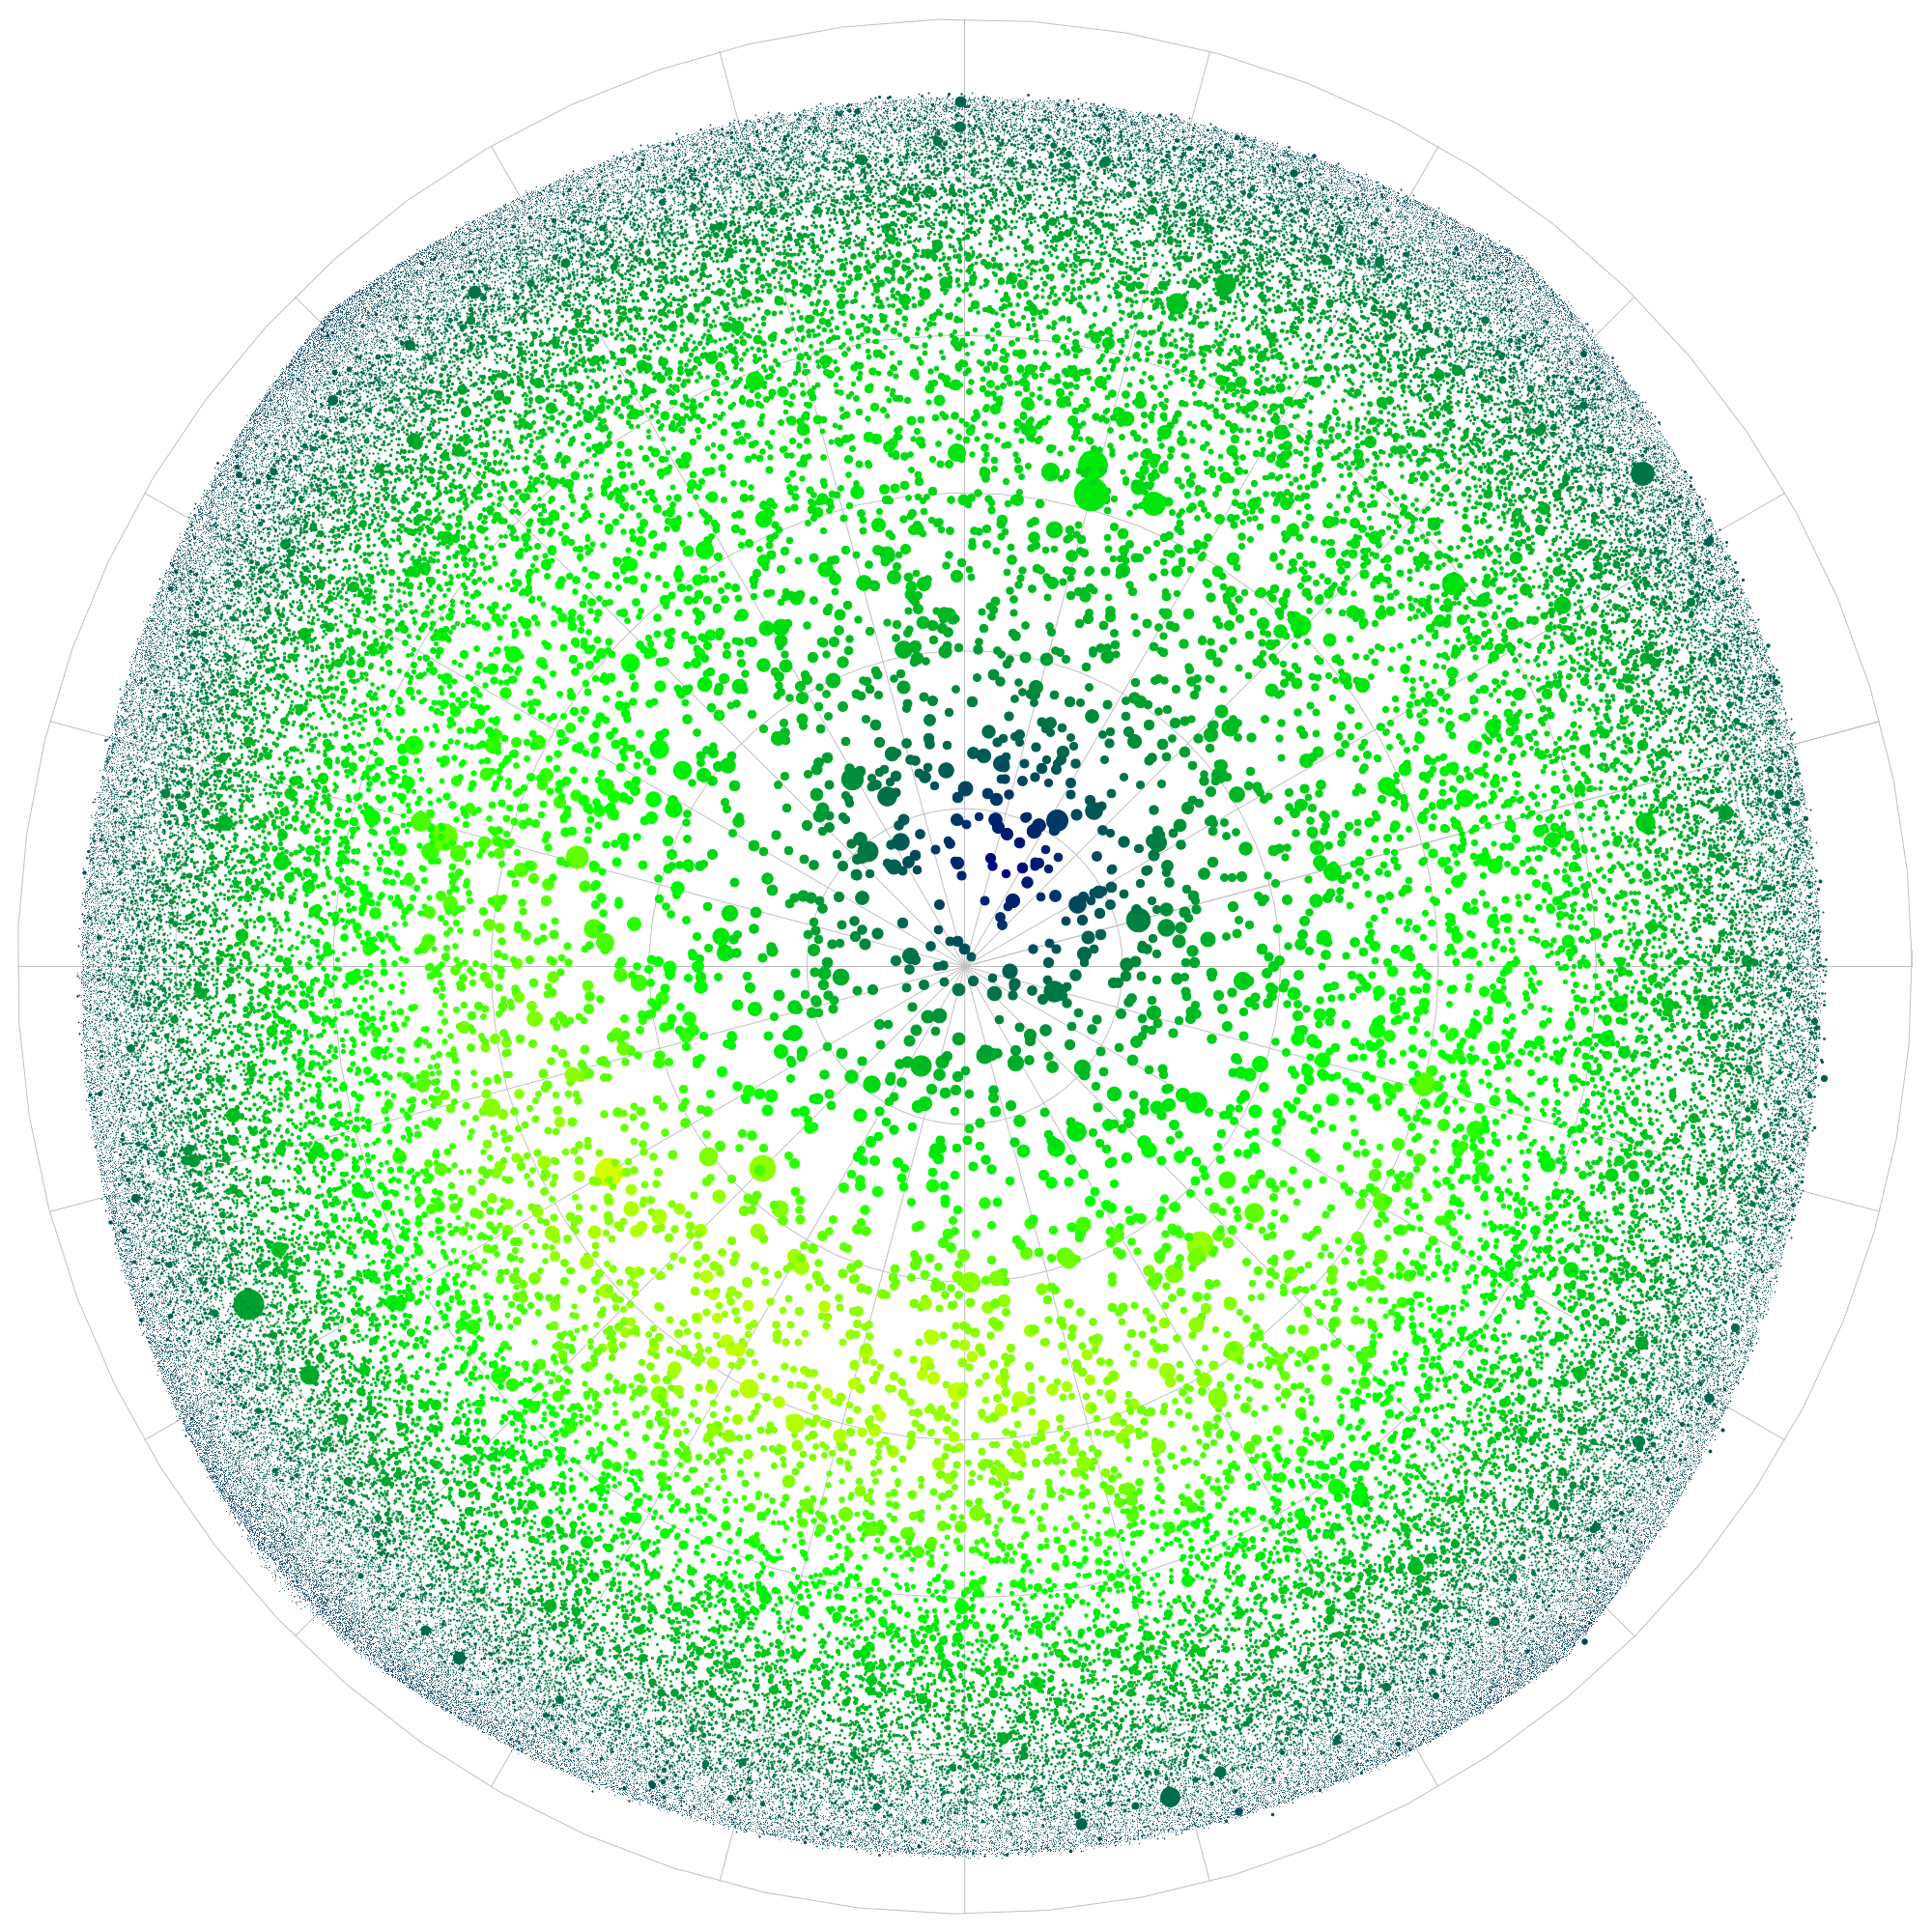
\includegraphics[width = \linewidth]{pictures/angularSpeed-ago.png}
        \caption{A set of 131072 meteors as observed from AGO Modra. Only the brightest frame is displayed for every meteor.
            Size of the dots represents the maximum brightness. Brighter colours correspond to higher observed angular speeds:
            meteors close to the horizon are at large distances, while velocities of meteors observed near the radiant have
            small radial components. Angular speeds are generally highest \ang{90} from the radiant.}
        \label{sim:res:as:as-ago}
    \end{figure}
    
    \begin{figure}
        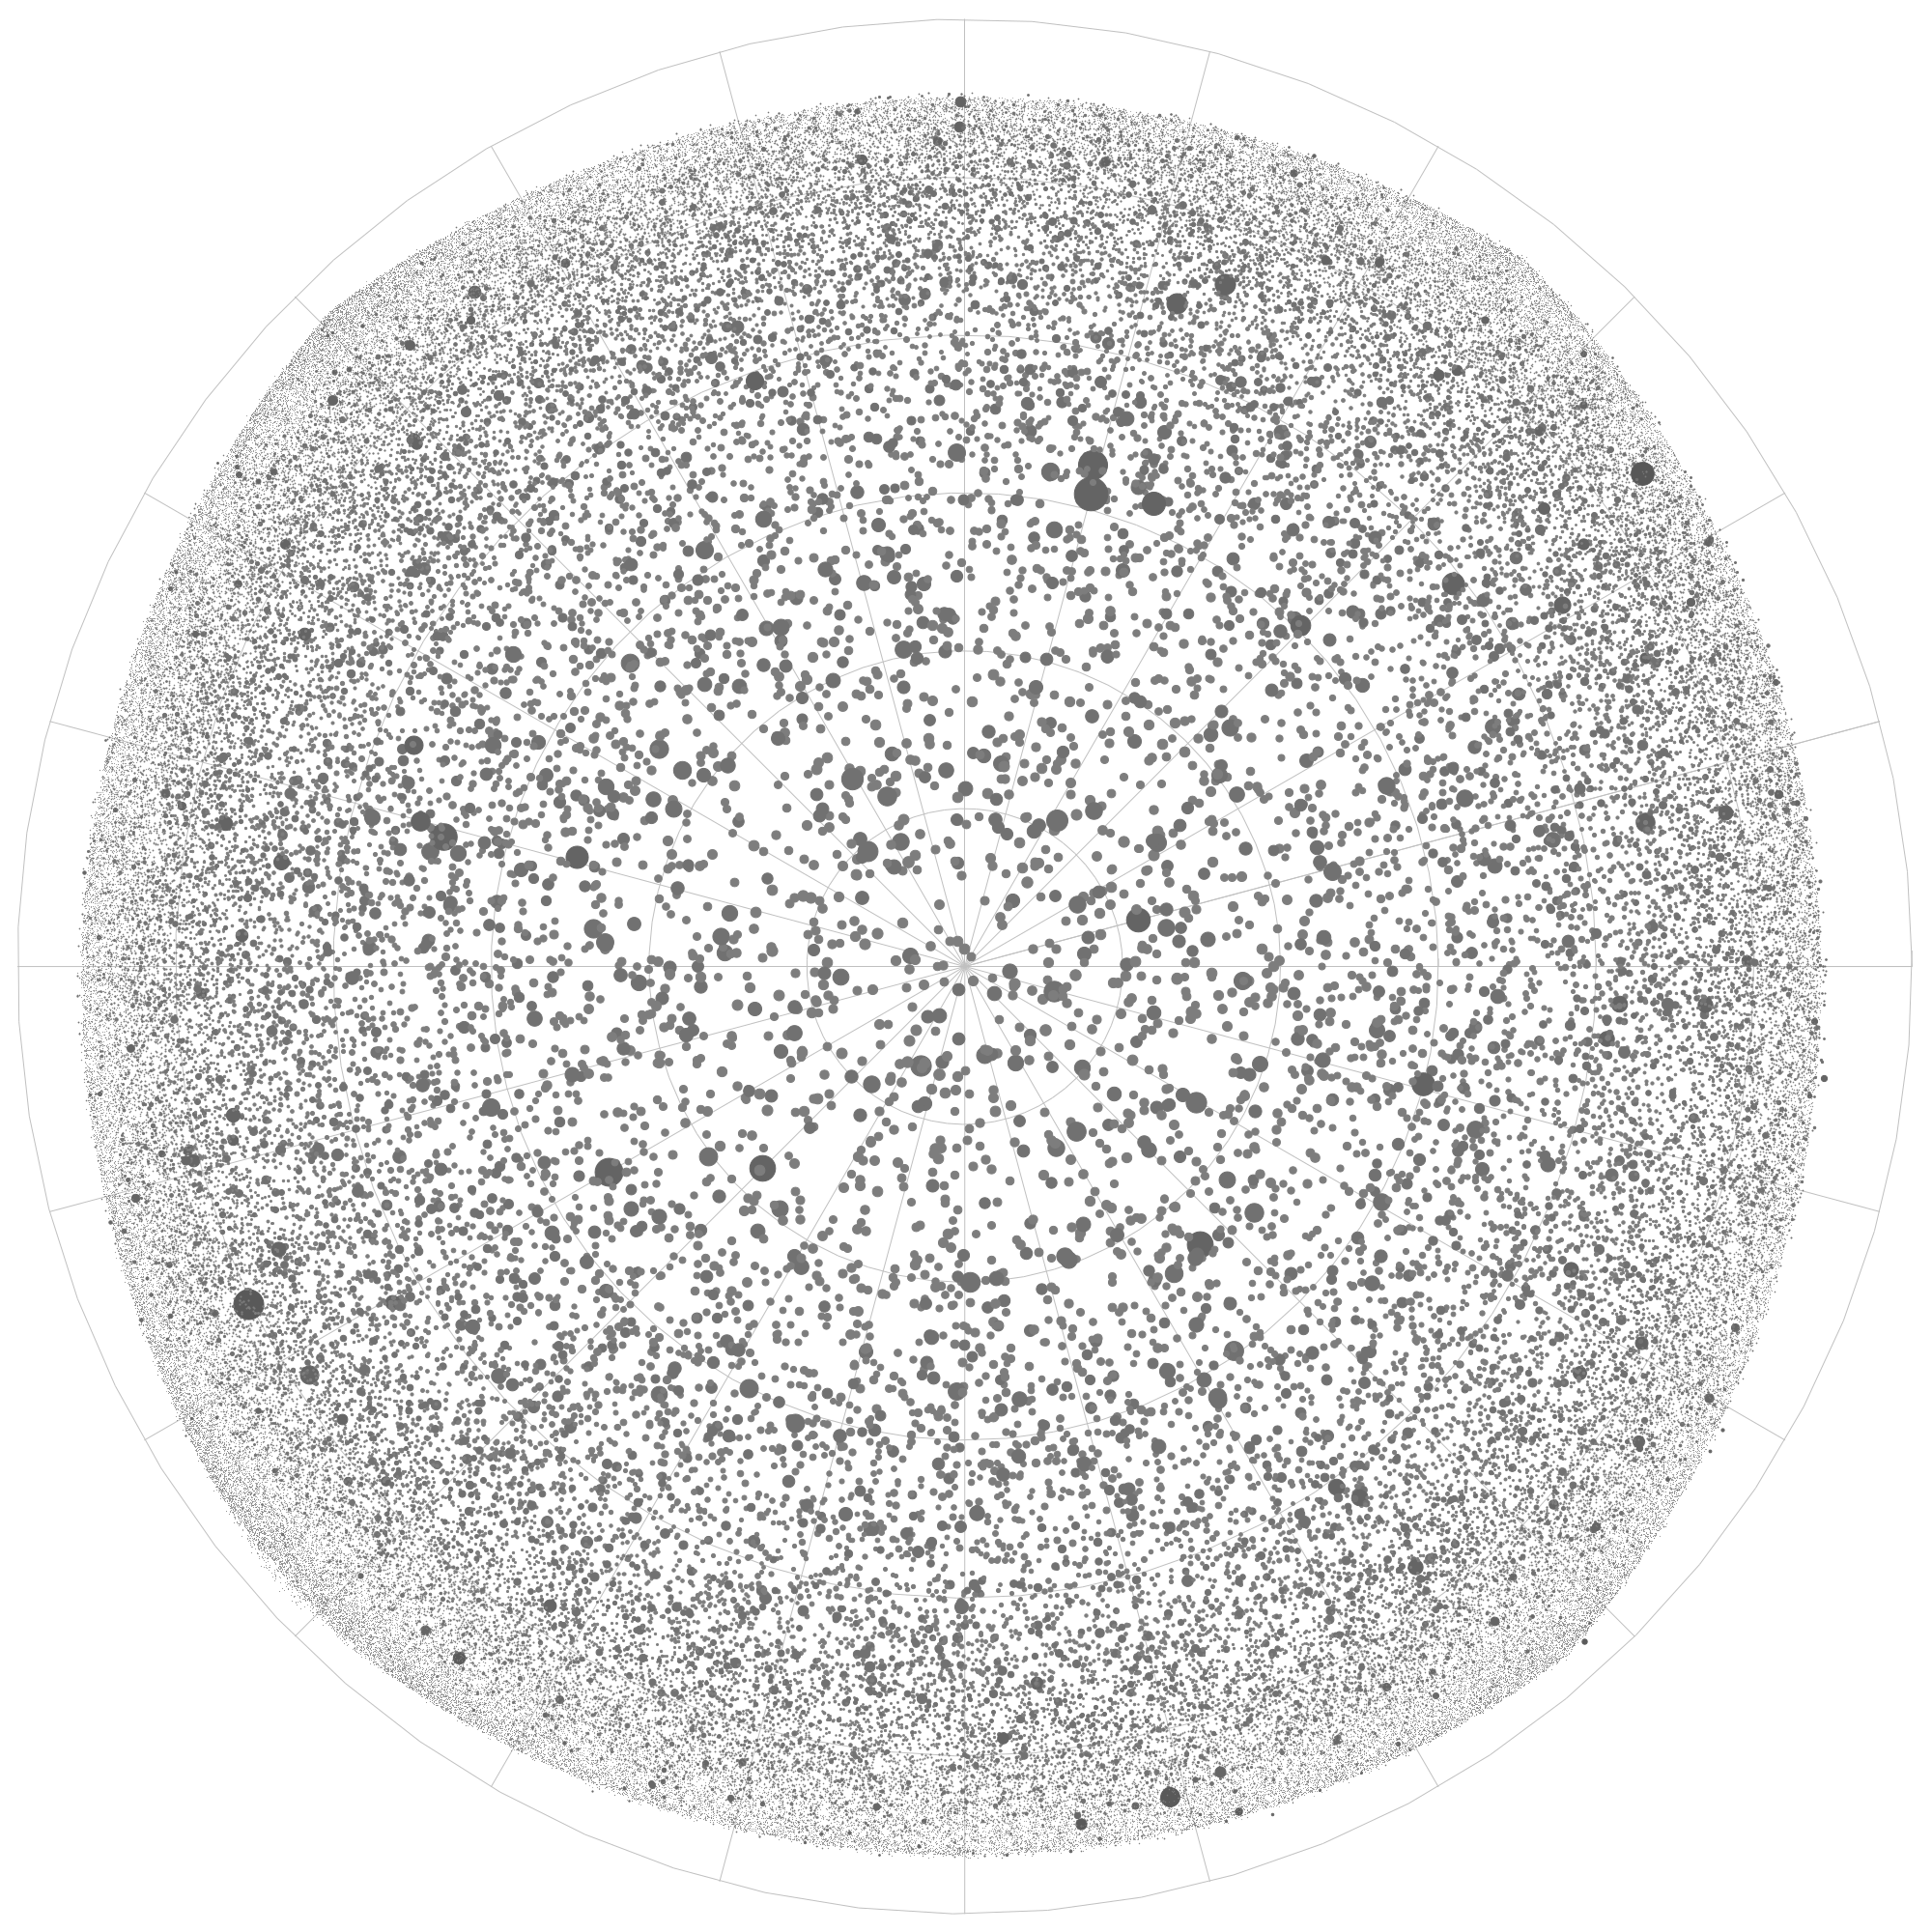
\includegraphics[width = \linewidth]{pictures/elevation-ago.png}
        \caption{The same dataset, coloured by elevation of the meteoroid at the time of maximum brightness. Darker dots represent lower elevations
            and thus generally correspond to larger particles at greater penetration depths.}
        \label{sim:res:as:ele-ago}
    \end{figure}

\input{conclusion.tex}






\section{Method}

    \subsection{Calibration of AMOS cameras}

    we are able to isolate a small change in velocity
    and mass, which can be used directly in the numerical integration:
    \begin{equation}
        \mathrm{d}v = -\frac{\Gamma A \rho_{\mathrm{air}} v^2}{m^{1/3} \rho^{2/3}} \mathrm{d}t\text{,}
        \label{eq:mc-dv}
    \end{equation}
    
    and a change of mass due to ablation as
    \begin{equation}
        \mathrm{d}m = -\frac{\Lambda}{2Q} \frac{Am^{2/3}}{\rho^{2/3}} \rho_{\mathrm{air}} v^3 \mathrm{d}t\text{.}
        \label{eq:mc-dm}
    \end{equation}
    
    where
    \begin{description}
        \item[$\Lambda$] is a dimensionless heat transfer coefficient,
        \item[$A$] is a dimensionless coefficient of shape
    \end{description}
    
    Typical values of $\Lambda$ and $A$ are on the order of unity. The value of $\Gamma$ also depends on the properties 
    of the environment, such as viscosity or density.
    For a spherical body in a flow with Reynolds number $10^4$ a value of $\Gamma \approx num{0.47}$ is used.
    
    \cite{jones-halliday2001} defined the excitation coefficient~$\zeta$, which represents
    the sum of all excitation probabilities over collisions and obtained the following relationship between $\zeta$ and $\tau$:
    \begin{equation}
        \tau = \frac{2\epsilon\zeta}{mv^2}\text{,}
        \label{m-tau}
    \end{equation}

    where $\epsilon$ is the mean excitation energy. For estimation of $\zeta$ we used a slightly improved version of the
    model compiled by \cite{hill2005}. In the formulae speed $v$ is stated in metres per second.
    To obtain the total flux of emitted visible light $F_0$, we take the time derivative of the particle's kinetic energy.
    Neglecting the second (deceleration) term yields the following \emph{equation of luminance}:
    \begin{equation}
        F_0 = \tau(v) \frac{\Lambda}{4Q} \rho_{\mathrm{air}} v^5\text{.}
        \label{m-f0}
    \end{equation}

    With this knowledge we are able to calculate the total luminous power of the meteor and subsequently its absolute magnitude.

\section{Simulation}
    
    \subsection{Generating the population}
    spherical earth
    
    \subsection{Observations}
    

\section{Physics of meteor flight} \label{sim:pmf}
    The analysis begins with detailed understanding of the physics of meteor flight in the upper atmosphere.
    /
    However, the used model needs to be reasonably simple and only replaced by a more 
    once there is an obvious reason to do so.
    
    \subsection{Equations of motion}            
        We use the standard model of meteor atmospheric flight developed by \cite{opik1958}.
        
        Since the simulation is primarily used to simulate small particles that ablate completely in the atmosphere,
        we do not need to account for meteoroid fragmentation 
        
        Hence, we only assume spherical particles
    
        \subsubsection{Braking equation} \label{sim:pmf:em:be}
            While atmosphere exerts a multitude of forces on the entering meteoroid particle,
            they are dominated by the drag force, acting in the direction opposite to the meteoroid's velocity vector.

            For small bodies at high velocities the influence of the Earth's gravity is negligible, 
            as they burn completely in a very short time. Forces with components perpendicular
            to the direction of the flight, such as aerodynamic lift or rocket effect caused by outgassing,
            can also be ignored. These assumptions are justified as long as we constrain the simulation to small particles which
            do not survive the atmospheric entry, and only consider entry speeds greater than the
            escape speed at any given altitude. Both conditions hold very well for meteoroid particles observed by
            intensified CCD cameras.

            Thus, for the purpose of the simulation we assume that each meteoroid particle always moves in a straight line
            and is only subject to deceleration caused by aerodynamic drag. We consider the standard form of the
            aerodynamic drag equation:
            \begin{equation}
                ma \equiv m\dot{v} = -\Gamma S \rho_{\mathrm{air}} v^2\text{,}
                \label{sim:pmf:em:be:ma}
            \end{equation}

            where
            \begin{itemize}
                \item $m$ is the instantaneous mass of the meteoroid particle (\si{\kilo\gram}),
                \item $\Gamma$ is the drag coefficient (dimensionless),
                \item $S$ is the cross-sectional area of the particle in the plane perpendicular to its velocity vector (\si{\metre\squared}),
                \item $v$ is its speed relative to the surrounding medium (\si{\metre\per\second}).
            \end{itemize}

            Note that while $\Gamma$ represents the shape of the particle, it is not constant during the flight.
            It also depends on the properties of the particle's surface, its attitude and various properties of the environment,
            such as Reynolds number (the ratio of inertial and viscous forces acting on the fluid surrounding the particle),
            air density and pressure. Its typical values are on the order of unity.
            $\Gamma \approx \num{0.47}$ corresponds to a spherical body in a flow with Reynolds number $10^4$.
            Values between \num{0.4} and \num{0.8} are typical for real meteoroid particles.

            We may express $S$ in terms of a dimensionless \emph{coefficient of shape} $A$, which is independent of the size of the particle;
            mass of the particle $m$ and its (constant) density $\rho$. This means that explicitly calculating the cross-sectional
            area is no longer necessary during the simulation.
            \begin{equation}
                S = A V^{2/3} = \frac{A m^{2/3}}{\rho^{2/3}}\text{,}
                \label{sim:pmf:be:S}
            \end{equation}

            where $V$ denotes the particle's volume. After dividing by $m$, equation \ref{sim:pmf:be:ma} takes the form
            \begin{equation}
                \mathrm{d}v = - \frac{\Gamma A}{m^{1/3}\rho^{2/3}}\rho_{\mathrm{air}} v^2\text{.}
                \label{sim:pmf:be:dotv}
            \end{equation}

            If the atmosphere is calm, $v$ is always equal to the magnitude of the particle's geocentric velocity $\vec{v}$.
            With meteors this assumption is well justified, since $v_{\mathrm{air}} \ll v$.
            Finally, for the purposes of the integrator a small change of velocity $\mathrm{d}v$ can be isolated:
            \begin{equation}
                \mathrm{d}v = -\frac{\Gamma A \rho_{\mathrm{air}} v^2}{m^{1/3} \rho^{2/3}} \mathrm{d}t\text{.}
                \label{sim:pmf:be:dv}
            \end{equation}

        \subsubsection{Equation of ablation} \label{sim:pmf:ea}
            In the model we assume that all of the available kinetic energy is converted to thermal energy and used
            to evaporate the material of the particle. This approximation is justified as long as the specific heat
            of vaporization is much greater than the thermal capacity of surrounding air. The equation takes the form
            \begin{equation}
                \dot{m} = -\frac{\Lambda}{2Q} S \rho_{\mathrm{air}} v^3\text{,}
                \label{sim:pmf:ea:dotm}
            \end{equation}

            where
            \begin{itemize}
                \item $\Lambda$ is the heat transfer coefficient (dimensionless);
                \item $Q$ is the specific enthalpy of vaporisation of meteoroid material
                    ($\si{\joule\per\kilo\gram} \equiv \si{\metre\squared\per\second\squared}$).
            \end{itemize}

            In real objects most of these quantities vary wildly on scales far smaller than the typical dimension of the particle.
            Naturally, such precision is meaningless in the simulation, so only constant values are considered. Either fixed mean values
            are used for the entire simulation, or each new particle is assigned a value randomly drawn from
            a pre-defined probability distribution. This is particularly important when generating particle masses.

            Once again, for the numerical simulation we need to isolate the change of mass $\mathrm{d}m$
            in a small time interval $\mathrm{d}t$:
            \begin{equation}
                \mathrm{d}m = -\frac{\Lambda}{2Q} \frac{Am^{2/3}}{\rho^{2/3}} \rho_{\mathrm{air}} v^3 \mathrm{d}t\text{.}
                \label{sim:pmf:ea:dm2}
            \end{equation}

        \subsubsection{Equation of luminance} \label{sim:pmf:el}
            In order to determine the apparent brightness of a simulated meteor, its absolute brightness must be calculated first.
            For the sake of simplicity we assume a constant fraction of total released energy is emitted as visible light,
            as opposed to energy lost to the atmosphere or consumed in heating and evaporating the body:
            \begin{equation}
                \Phi_e \propto \frac{\mathrm{d}E_\mathrm{kin}}{\mathrm{d}t}\text{.}
                \label{sim:eq:lum:dekin}
            \end{equation}

            where $\Phi_e$ denotes the total isotropic \emph{radiant flux} over all visible wavelengths of the elecromagnetic spectrum.

            The constant of proportionality is usually denoted $\tau$ and named \emph{luminous efficiency factor} \cite{hill2005}.
            Most of the particle's kinetic energy is transformed
            to heat and ionization of atoms and only a very small fraction is emitted as visible light.
            Luminous efficiency is usually considered to be a function of speed and
            meteoroid material \cite{jones-halliday2001}. Since we assume a homogeneous composition for each meteoroid,
            in each flight simulation $\tau$ is solely a function of speed and as such must be recomputed in every integration step.
            Its typical values are on the order of $10^{-2}$.

    \subsection{Supplementary quantities} \label{s}
        In addition to the properties of the meteoroid particle itself, the simulator needs to know various
        properties of the environment or the observer.

        \subsubsection{Atmospheric density}
            The density of the air $\rho_{\mathrm{air}}$ appears in all of the above equations
            and must be calculated before any equations of motion can be solved.
            At the altitudes where meteors occur the standard isothermal approximation no longer holds.\footnote{At \SI{100}{\kilo\metre},
            isothermal atmosphere overestimates density by a whole order of magnitude compared to the output of
            a high-precision model \cite{msise90}.} Therefore it is necessary to use a more precise model.
            
            High-order polynomial fitting atmospheric models, such as those found in \cite{braeunig2014} and \cite{ussa1976}, are sufficiently precise,
            however, since air density must be calculated in every iteration of the integrator, their use is prohibitively expensive.

            In order to reduce computation time we used a simple and fast tabular approximation of the
            NASA Mass-Spectrometer-Incoherent-Scatter Extended 1990 (MSIS-E-90) atmosphere model \cite{msise90}.
            Values were tabulated by \SI{1}{\kilo\metre} and interpolated by a piecewise exponential function.
            The results of this approximation differ from true values in the model less than one part in ten thousand,
            which greatly exceeds the required precision.

        \subsubsection{Air mass} \label{sim:pmf:sq:am}
            Air mass calculation is crucial for determining the effects of atmospheric extinction.
            It is perfectly reasonable to use the same function as in \ref{fwd:nbs:opt:ae}.
            Since magnitude scale is logarithmic in nature and the decrease in brightness in exponential,
            the resulting increase in apparent magnitude is linearly proportional to optical thickness, which is in turn
            linearly proportional to air mass.

        \subsubsection{Coordinate transformations} \label{sim:pmf:sq:ct}
            To achieve highest precision \textsc{Astropy}'s built-in \texttt{EarthLocation} class should be used.
            The positions are internally represented as three-dimensional Cartesian vectors. Human-readable output
            and altitude calculations are obtained after transforming the coordinates to \texttt{WGS84} geoid.

            However, computation time can be drastically reduced if the Earth is modelled as a sphere. Since
            flattening of the Earth spheroid is only approximately $1/298$ \cite{nima2000}, this approximation does not
            result in significant errors compared to other simplifications we have already made.
            It should be noted that the error also depends on the distance between the meteor and the observer,
            which is always much less than the radius of the Earth; and the total error is thus negligible.

        \subsubsection{Angular speed} \label{sim:pmf:sq:as}
            The calculation of perceived brightness also requires taking angular speed into account.
            Light from faster meteors is spread on a larger number of CCD pixels,
            lowering the signal-to-noise ratio and thus also the probability of a successful detection.

            In context of meteor motion, angular speed means the apparent length of the projection of the meteor's
            true velocity vector onto the celestial sphere.
            Let us denote this vector $\vec{v}$ and let $\vec{r}$ be the position of the meteoroid with respect to the observer.
            The projection onto a spherical sky can be represented as the projection onto a plane perpendicular to $\vec{r}$ and
            passing through the meteoroid, which we will denote $\mathrm{rej}_{\vec{r}}\vec{v}$.%
            \footnote{The projection of $\vec{v}$ onto the plane perpendicular to $\vec{r}$ is also called the \emph{rejection}
            of $\vec{v}$ onto $\vec{r}$ \cite{perwass2008}.}
            
            For any two vectors $\vec{r}$ and $\vec{v}$, $\vec{v}$ is the sum of its projection and rejection onto $\vec{r}$:
            \begin{equation}
                \mathrm{proj}_{\vec{r}}\vec{v} + \mathrm{rej}_{\vec{r}}\vec{v} = \vec{v}\text{.}
                \label{sim:pmf:sq:as:rej}
            \end{equation}
            
            The projection vector can be obtained easily using dot product as
            \begin{equation}
                \mathrm{proj}_{\vec{r}}\vec{v} = \frac{\vec{r}\cdot\vec{v}}{r} \cdot \frac{\vec{r}}{r} = \frac{\vec{r}\cdot\vec{v}}{r^2}\vec{r}\text{.}            
                \label{sim:pmf:sq:as:proj}
            \end{equation}
            
            Putting these equations together we obtain the formula for apparent angular speed,
            \begin{equation}
                \omega = \frac{\left|\vec{v} - \frac{\vec{r}\cdot\vec{v}}{r^2}\vec{r}\right|}{r}\text{.}
                \label{sim:pmf:sq:as:asf}
            \end{equation}

\section{Algorithm}
    With full knowledge of underlying equations, we may proceed to designing the simulation algorithm.

    \subsection{Generating the meteoroids}
        The first step of the simulation is to create the initial population of meteoroid particles entering the atmosphere.
        At this point, we pretend not to know anything about observers and are only concerned with
        physical representations of virtual meteoroid objects.
        
        To reduce the size of the possible parameter space, we fixed the values of most
        parameters that are known CITE THIS or can be determined experimentally, such as the        
        \begin{itemize}
            \item heat transfer coefficient $\lambda$ (\num{0.5}),
            \item specific heat of vaporizarion $Q$ (\SI{8}{\mega\joule\per\kilo\gram}),
            \item coefficient of shape (\num{0.47}).
        \end{itemize}

        In \textsc{Asmodeus}, this process in handled by the script \texttt{asmodeus-generate.py}.
        
        \subsubsection{Initial masses}
            First of all the particles are assigned their initial mass. Meteor showers are typically described
            by the \textbf{mass population index} $s$. The differential spectrum of masses follows a power law:
            \begin{equation}
                N(m) = m^{-s}\text{,}
            \end{equation}
            
            with typical values of $s$ being \numrange{1.5}{2.5}. Since this distribution is divergent for $m \to 0$,
            we also need to establish the lower bound on meteor masses $m_\mathrm{min}$. This requirement effectively yields
            a Pareto I distribution with $s$ as the parameter of scale and $m_\mathrm{min}$ as the XXXXXXX.
            
            have a look at this again
            
        \subsubsection{Initial positions}
            Each meteoroid particle is assigned a starting position within a predefined geographic area. Its precise bounds
            are not important and may be chosen somewhat arbitrarily, as long as several conditions hold:        
            \begin{itemize}
                \item The entire sky visible from each station must be covered. Setting the bounds too close to the observers
                    will result in less generated meteors in that direction, especially near the horizon. This would
                    introduce undesirable skewing to the observed distribution.
                \item The total area should be as small as possible. If the area is too large, most meteors will be never registered
                    after atmospheric extinction and other effects are applied, while the required computation time
                    stays roughly the same as with registered meteors.
                \item The shape of the area should be simple. Sampling the source distribution should be a straightforward process.
            \end{itemize}
        
            Setting an artificial limit on the statistics, for instance requiring the altitude to be at least \ang{15},
            simplifies fulfilling these conditions significantly. The minimum required area is also easier to calculate this way.

            Two simplest shapes are a spherical rectangle\footnote{By this we mean a true \emph{rectangle}, ie. a figure with four right angles,
            bounded by two parallels and two meridians. ``Spherical rectangle'' usually refers to a shape whose
            four angles are equal, but necessarily larger than \ang{90}.} and a circle.
            A slight disadvantage of the rectangle is that the distribution cannot be sampled as two independent
            uniform distributions, since this would result in more meteoroids being generated at the side closer to the pole.

            This excess can be described in terms of geographic latitude $\phi$. On a spherical Earth
            the length of a parallel is equal to $R \cos{\phi}$: if meteoroid longitudes are sampled
            from a uniform distribution, the excess will be proportional to $\frac{1}{\cos\phi}$.
            
            To correct the distribution and obtain a constant particle density of the entire covered part
            of the surface, we might discard the excess meteoroids immediately. This can be achieved simply
            by only accepting particles with probability $p_a$, proportional to the length of th intersection
            of the parallel where the meteoroid was placed upon generation:
            \begin{equation}
                p_a(\phi) = \cos\phi\text{.}
                \label{sim:al:gtm:ip:proba}
            \end{equation}
            
            A slight performance increase can be achieved by normalizing the density to the
            length of the parallel closest to the equator. All meteoroids generated at this boundary will be accepted,
            resulting in less wasted computation time.
            Equation \ref{sim:al:gtm:ip:proba} then transforms to
            \begin{equation}
                p_a(\phi) = \frac{\cos\phi}{\cos\phi_0}\text{,}
                \label{sim:al:gtm:ip:prob2}
            \end{equation}

            where $\phi_0$ is the latitude of the parallel closest to the equator.
            
            For meteor showers we also need to include the effects of the altitude of the radiant.
            Higher altitudes (or conversely, lower zenith distances) result in a larger effective projection area.
            The effect is proportional to the sine of the radiant altitude.
            
            Once again, we may solve this by accepting generated meteors with a certain probability $p_r$,
            which varies with altitude of the radiant at the time of the atmospheric entry at
            the position of the meteor above the Earth's surface.
            Of course, it must be computed for each meteor independently.
            \begin{equation}
                p_r = \cos\theta_r(\phi, \lambda, t)\text{,} 
                \label{sim:al:gtm:ip:probr}
            \end{equation}
            
            where
            \begin{itemize}
                \item $\theta_r$ is the altitude of the radiant,
                \item $\phi$ is the latitude of the meteoroid particle,
                \item $\lambda$ is the longitude of the meteoroid particle,
                \item and $t$ is the time of the entry.
            \end{itemize}
            
            The probability that a generated meteoroid will be accepted and simulated
            is determined by the product of probabilities \ref{sim:al:gtm:ip:prob2} and \ref{sim:al:gtm:ip:probr}.           
           

        \subsubsection{Initial velocities} \label{sim:al:gm:iv}
            In the next step we need to assign the particles their initial velocities.
            There are two distinct approaches to this problem, depending on whether
            the program simulates a particular \emph{meteor shower} or the \emph{sporadic background}.
            
            Simulating the sporadic background would be significantly more challenging. The apex, antapex and anthelion
            sources present different flux densities, which change with time and location.
            With meteor showers the situation is substantially simpler: all particles share a common parent
            body, which translates to a common radiant and similar atmospheric entry speeds.
            On the contrary, sporadic background exhibits a relatively constant average flux,
            while intensities of meteor showers vary considerably even on short time scales.
            
            Naturally, the real observed distribution includes both sources simultaneously.
            In the simulation we only considered meteor showers with constant radiant
            with respect to the geocentric equatorial coordinate system.
            The transformation to an ECEF\footnote{Earth-centered, Earth-fixed -- a terrestrial coordinate system, rotating with the Earth,
            as opposed to a nonrotating celestial coordinate system} coordinate system is fairly straightforward
            and already implemented in \textsc{Astropy}.
                        
            Note that while initial velocities of the particles in the simulation are not equal to their true geocentric velocities,
            as would be observed outside the gravitational influence of the Earth.
            
            Simulations of sporadic background meteors are also planned once the system is tested.

        \subsubsection{Atmospheric entry}
            Once the initial position is deemed acceptable, atmospheric entry may be simulated and recorded.            
            In \ref{sim:pmf} we obtained a system of interdependent differential equations,
            which can be solved numerically.
            
            Two solver have been evaluated. The semi-implicit Euler integrator is much easier to
            implement and requires significantly less time to evaluate one step, but requires a large number
            of steps to achieve sufficient precision.

            A fourth-order Runge-Kutta solver is more precise but also more difficult to implement,
            especially since the mass of the meteoroid is changing during the simulation.
            Considerable effort has been made to ensure the solver produces correct results.
            
            The frequency of the captured frames is equal to the frame rate of real AMOS cameras.
            In Slovakia, the frame rate is fixed at 15 frames per second.            
            This does not necessarily equal the time step taken by the integrators,
            as multiple small steps may be taken between two successive frames.
            The interpolating steps are discarded and only 15 frames per second
            are selected for further analysis.
            
            In practice, we found that the precision of RK4 integrator does not
            increase noticeably if time step is set to less than 1/75 of a second
            while computation time is still acceptable. 
            
            If higher precision
            
    \subsection{Processing the observations} \label{sim:al:po}
        In the next step each meteoroid is \emph{observed} -- its projection on the sky
        is computed for each of the observing stations, along with its apparent luminosity
        and other important properties as observed in each frame.
        
        \subsubsection{Calculation of projection}
            Meteor projections are computed independently for each observer.
            The geographic coordinates are first transformed to an observer-centered altitude-azimuthal coordinate system.
            As a spherical Earth model is used, this is done easily by several matrix transforms.            
            AMOS cameras project the sky in an equidistant polar projection: each degree of altitude is
            transformed to an equal radial distance on the CCD. This simplifies plotting
            the observed meteors, as a 2D polar chart may be used without any further adjustments.
            
            To establish the apparent brightness, luminous flux at the location of the observer is calculated.
            The total luminous power in each frame is reduced to the surface of a sphere with radius equal
            to the distance between the frame and the observer to obtain luminous flux in watts per square metre:
            \begin{equation}
                I \propto d^{-2}\text{.}
                \label{sim:al:po:cp:d}
            \end{equation}
            
            This value is further reduced by atmospheric extinction. Extinction is described in terms of \textbf{relative air mass} $X$,
            which is a dimensionless quantity that specifies the ratio of optical thickness in the direction of the observed
            object to the optical thickness in zenith:
            \begin{equation}
                X = \frac{%
                    \int\limits_{\text{observer}}^{\text{zenith}} \kappa(s)\rho_{\mathrm{air}}(s) \mathrm{d}s%
                }{%
                    \int\limits_{\text{observer}}^{\text{object}} \kappa(s)\rho_{\mathrm{air}}(s) \mathrm{d}s%
                }\text{.}
                \label{sim:al:po:cp:airmass}
            \end{equation}
            
            High precision air mass models have been developed, such as \cite{kasten-young1989}.
            The decrease in brightness increases exponentially with optical thickness as $e^{-kX}$ for some constant $k$.
            This constant must be determined experimentally. If we assume that the atmospheric effects make
            a meteor in zenith $(X = 1)$ appear about \SI{25}{\percent} dimmer, $k$ must be equal to
            $-\ln \left(1 - 0.2\right) \approx 0.288$.
            
        \subsubsection{Application of selection bias}
            After all natural effects have been applied and apparent position and magnitude have been computed,
            we need to simulate the instrumental effects, introduced by the detection apparatus.
            
            Various sources of selection bias 
            For further details refer to \cite{balaz-inprep}.
            
            We assumed a sigmoid profile of the detection efficiency curve:
            \begin{equation}
                D(m) = \frac{f}{1 + e^{\frac{m - m_0}{\omega}}}\text{.}
                \label{eq:sls}
            \end{equation}
            
            where
            \begin{itemize}
                \item $m_0$ is the limiting magnitude, defined as the point where
                    detection efficiency is equal to half of its maximal value.
                \item $\omega$ denotes the width of the distribution.
                    Smaller values correspond to a sharp detection efficiency falloff.
                \item $f$ is the \emph{fill factor}: the upper limit of the system's detection ability.
                    Random occurrences, such as discriminator failures, power outages and similar problems
                    may prevent detection even under otherwise perfect conditions. Thus even for very
                    bright bolides detection is not always assured.
            \end{itemize}

            The exact shape of the detection efficiency profile was derived from observational data.
            In the dimmer part of the apparent luminosity spectrum ($-2^\mathrm{m}$--$5^\mathrm{m}$),
            two nights of simultaneous observations by two AMOS cameras and seven human observers were analyzed.
            Only meteors captured by human observers were taken into account. We investigated all visual meteor records
            and paired them with automated records by timestamps. The fraction of meteors captured by AMOS
            was recorded 
            
            These data did not include any meteors brighter than $-2^{\mathrm{m}}$.           
            Bolide data were obtained from long-term simultaneous observations with AMOS cameras and photographic
            plates at AGO Modra. We asserted that the photographic plate is a perfect observer and searched for corresponding
            records in AMOS databases. Again, we ignored all AMOS reports of bolides that were not captured on photographic plates.
            The data were collected at AGO Modra between 2010 and 2016. AMOS registered 57 out of 67 bolides recorded on
            the plates.

            After putting both data sources together we fitted the observed distribution with function \ref{sim:al:po:asb:dm}.
            
            \begin{figure}
                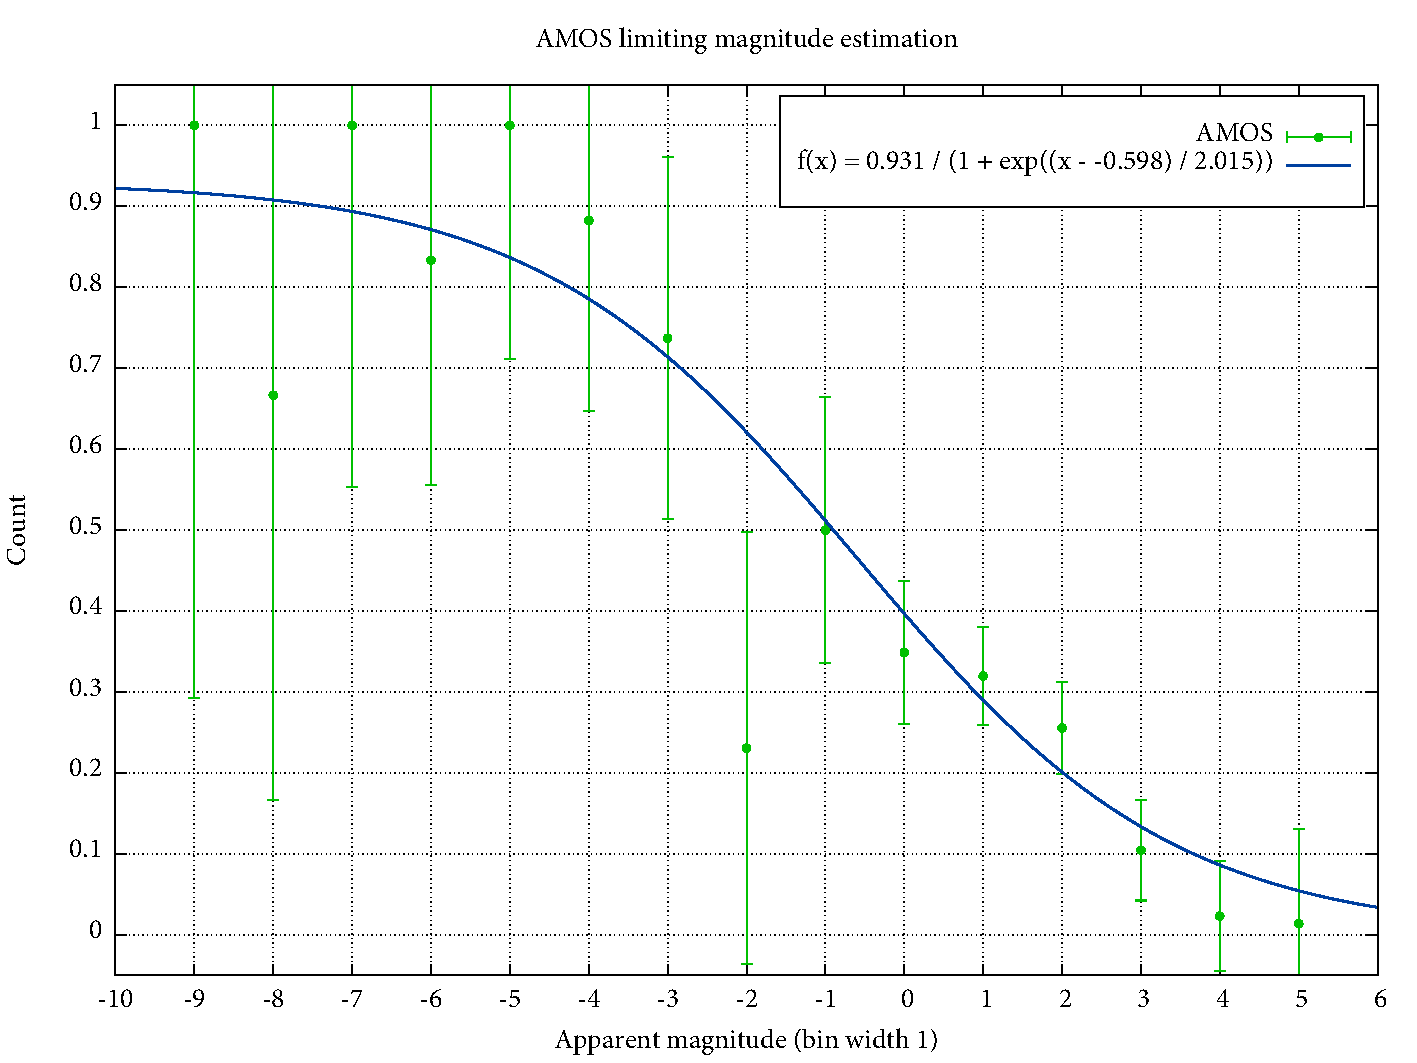
\includegraphics[width = \linewidth]{pictures/limmag.pdf}
                \caption{Detection efficiency falloff curve.
                    Bin width $1^\mathrm{m}$, error bar size is $\frac{1}{\sqrt{N + 1}}$, where $N$ is the number of observed meteors in the bin.
                    Limiting magnitude is $\mu \doteq \num{-0.6}$, falloff rate is $\omega \doteq \num{2}$, and fill factor reaches
                    over \SI{93}{\percent}.
                }
                \label{sim:al:po:limmag}
            \end{figure}

\section{\textsc{Asmodeus}}
    The described algorithm has been implemented and tested in a suite of scripts named \textsc{Asmodeus}.
    The name is a free acronym of \textbf{A}ll-\textbf{s}ky \textbf{M}eteor \textbf{O}ptical
    \textbf{D}etection \textbf{E}fficiency \textbf{S}im\textbf{u}lator.
    \textsc{Asmodeus} is written in Python 3 and uses the \textsc{Astropy} library.

    \subsection{Operation} \label{sim:op}
        First, configuration data are loaded from the specified file in \texttt{YAML} format.
        Certain parameters may be overridden using command-line arguments.

        \texttt{N} meteors are then simulated. Each meteor is assigned a starting position within predefined
        geographic coordinates at a fixed altitude of \SI{150}{\kilo\metre}, and a geocentric velocity vector.
        Positions are sampled from a uniform distribution. For a meteor shower, the velocity vector components
        are constant in the equatorial coordinate system.



\begin{acknowledgements}
    This work has been supported by the special stipendium provided by FMPH CU (October 2017), UK grant number 123456
\end{acknowledgements}


%-------------------------------------------------------------------

\bibliographystyle{aa}
\bibliography{references.bib}

\end{document}
